% !TEX program = lualatex
% Cerema, 10 septembre 2026. Page de titre habituelle et cinq slides de contenu.
\pdfvariable objcompresslevel = 0
\documentclass[A4,svgnames,9pt,aspectratio=169]{beamer}
\usepackage[french]{babel}
\usepackage{amsmath,amssymb,amsfonts,mathtools}
\usepackage{graphicx}
\usepackage{tikz}
\usetikzlibrary{positioning,shapes,arrows.meta,calc,fit,backgrounds,babel,decorations.pathreplacing}
\usetheme{inria}
% Même substitution que dans la soutenance : petites capitales Latin Modern Roman.
\DeclareFontShape{TU}{lmss}{m}{sc}{<->ssub*lmr/m/sc}{}
\colorlet{inria-bleu}{inria-2024-bleu-azur}
\graphicspath{{figs/}}
\title[Réunion Inria--Cerema]{Réunion Inria--Cerema}
\subtitle{SAM gelé, LoRA et guidage hiérarchique}
\author[L. \textsc{Hauseux} \textit{et al.}]{\texorpdfstring{%
  {\small Inria, éq. \textsc{Ayana} : Louis \textsc{Hauseux}, Josiane \textsc{Zerubia}}\\
  {\small Cerema, éq. \textsc{Endsum} : Raphaël \textsc{Antoine}, Philippe \textsc{Foucher}, Pierre \textsc{Charbonnier}}%
}{Louis Hauseux, Josiane Zerubia, Raphaël Antoine, Philippe Foucher, Pierre Charbonnier}}
\institute{Inria, équipe \textsc{Ayana} ; Cerema, équipe \textsc{Endsum}}
\date[L.~Hauseux --- Cerema, 10 septembre 2026]{10 septembre 2026}
\hypersetup{allcolors=rouge_inria,
  pdfauthor={Louis Hauseux, Josiane Zerubia, Raphaël Antoine, Philippe Foucher, Pierre Charbonnier},
  pdftitle={SAM gelé, LoRA et guidage hiérarchique},
  pdfsubject={Présentation Cerema du 10 septembre 2026},
  pdfkeywords={SAM 2, LoRA, Frangi, hiérarchie, Graphormer, biais d'attention}}

% Pied de page du thème de soutenance ; le grand logo suffit sur la page de titre.
\setbeamertemplate{footline}{%
  \leavevmode\hspace*{\hmargin}%
  \raisebox{0.4\footerheight}{%
    \parbox{\dimexpr\paperwidth-2\hmargin}{%
      \textcolor{inria-noir}{\insertshortdate\hfill
      \ifnum\value{page}>1\relax
        \smash{\raisebox{-0.1\footerheight}{\footerlogo}}\kern2em
      \fi
      \insertframenumber/\inserttotalframenumber}}}}
\newcommand{\formulebox}[1]{%
  {\setlength{\fboxsep}{8pt}\setlength{\fboxrule}{0.8pt}%
   \fcolorbox{inria-rouge}{gray!4}{#1}}}
% Citation layout retained from the 2026-09-08 thesis defence.
% Load in the preamble, after the Inria theme and textpos/hyperref packages.
% BibTeX supplies declarations only: no bibliography slide is added.
\makeatletter
\newcommand{\DeclareRef}[3]{%
  \expandafter\gdef\csname ref@lab@#1\endcsname{#2}%
  \expandafter\gdef\csname ref@full@#1\endcsname{#3}}
\newcommand{\DeclareMyRef}[3]{\DeclareRef{#1}{#2}{#3}%
  \expandafter\gdef\csname ref@mine@#1\endcsname{}}
\newcommand{\refbracket}[1]{%
  \ifcsname ref@mine@#1\endcsname
    \textcolor{inria-rouge}{[\csname ref@lab@#1\endcsname]}%
  \else
    \textcolor{gris_fonce_inria}{[\csname ref@lab@#1\endcsname]}%
  \fi}
\newcommand{\citb}[1]{\mbox{{\footnotesize\bfseries\refbracket{#1}}}}
\newcommand{\bibligne}[1]{\item {\bfseries\refbracket{#1}}\ \csname ref@full@#1\endcsname}
\newcommand{\reffoot}[1]{%
  \begin{textblock}{0.90}[0,1](0.05,0.925)%
    \begingroup
    \tiny\linespread{0.90}\selectfont\raggedright\color{gris_fonce_inria}%
    \setlength{\parindent}{0pt}\setlength{\parskip}{0pt}%
    \edef\rf@list{\zap@space#1 \@empty}%
    \@for\rf@key:=\rf@list\do{%
      \noindent{\bfseries\expandafter\refbracket\expandafter{\rf@key}}%
      \space\csname ref@full@\rf@key\endcsname\par}%
    \endgroup
  \end{textblock}}
\makeatother

% Standard LaTeX \bibliography writes \bibdata and loads \jobname.bbl,
% including with -output-directory=build. Its first pass tolerates absence
% of the .bbl; running BibTeX and LaTeX twice supplies all labels and links.
% Register the keys directly: our declarations are not numbered \bibitem
% entries, so \nocite would incorrectly report undefined LaTeX citations.
\makeatletter
\AtBeginDocument{%
  \bibliographystyle{references}%
  \if@filesw
    \immediate\write\@auxout{\string\citation{ying21,euvip26,hu22,turaga09,ravi24}}%
  \fi
  \bibliography{references}%
}
\makeatother


\begin{document}
% Page de titre habituelle du thème Inria, ancrée à la page pour éviter
% les débordements de sa boîte pleine page dans la zone de contenu Beamer.
\begingroup
\setbeamertemplate{title page}{%
  \begin{tikzpicture}[remember picture,overlay]
    \node[anchor=north west,inner sep=0pt,outer sep=0pt]
      at ([xshift=\hmargin,yshift=-\vmargin+\titlelogovoffset]current page.north west)
      {\titlelogo};
    \node[anchor=north west,align=left,text=inria-noir,
      text width=.74\paperwidth,inner sep=0pt,outer sep=0pt]
      at ([xshift=\fullpageinnerhmargin+0.15\textwidth,yshift=-.34\paperheight]current page.north west)
      {{\Huge\textbf{\inserttitle}}\\
       {\barrecouleur}\\[2ex]
       {\Large\insertsubtitle}\\[3ex]
       {\insertauthor}};
  \end{tikzpicture}%
}
\frame{\titlepage}
\endgroup

% Adaptation de la slide 55 (page PDF 64) de la soutenance du 8 septembre 2026.
% Le constat vient de nos essais ; la redondance est une explication envisagée.
\begin{frame}[t]{Hessienne, gradient : le guidage n'a pas aidé}
  \begin{center}
    \resizebox{0.48\textwidth}{!}{\input{figs/lora_adaptation}}\par\smallskip
    {\small \textbf{Base : SAM gelé + LoRA} \citb{hu22}, comme dans CrackSAM \citb{ge24}.}
  \end{center}
  \vspace{0.10cm}
  \small
  \begin{itemize}
    \setlength{\itemsep}{7pt}
    \item \textbf{Nos essais :} ajouter la hessienne, le gradient ou Frangi
      \textbf{n'améliore pas} SAM + LoRA.
    \item \textbf{Explication possible :} ces informations locales semblent
      \textbf{déjà représentées par SAM}.
    \item \textbf{Limite de Frangi :} les ombres et la granularité
      provoquent des \textbf{sur-détections}.
  \end{itemize}
  \vspace{0.16cm}
  \begin{center}
    \formulebox{\parbox{0.83\textwidth}{\centering\small
      \textbf{Piste :} relier les zones d'une même fissure par une \textbf{hiérarchie}.}}
  \end{center}
  \reffoot{hu22,ge24}
\end{frame}

% Source: soutenance du 8 septembre 2026, reprise sans modification du contenu.
\begin{frame}[t]{Comment guider l'attention \emph{via} la hiérarchie ? Une idée à explorer}
    \vspace{0.02cm}
    \begin{center}
        \resizebox{0.64\textwidth}{!}{\input{figs/attention_biais}}
    \end{center}

    \vspace{0.06cm}
    \small
    \begin{itemize}
        \setlength{\itemsep}{3pt}
        \item L'\textbf{attention} : chaque jeton pose une \textbf{requête}, la compare aux
        \textbf{clefs} de tous les autres, et repart avec la moyenne de leurs \textbf{valeurs},
        pondérée par un \textbf{score visuel} que SAM sait déjà calculer
        \item On y \textbf{ajoute un bonus} avant le \emph{softmax} : un échange \textbf{favorisé},
        jamais imposé \citb{ying21}
        \item Le bonus vient de la \textbf{hiérarchie} du graphe de \textsc{Frangi} : plus deux jetons
        \textbf{fusionnent tôt} dans l'arbre, plus il est fort, même loin dans l'image \citb{euvip26} ;
        LoRA l'apprend avec un \textbf{seul} coefficient $\beta$ \citb{hu22}
    \end{itemize}

    \vspace{0.06cm}
    \begin{center}
        \formulebox{\parbox{0.80\textwidth}{\centering\small
        $\mathrm{attention} \;=\; \mathrm{softmax}\bigl(\text{scores visuels} \;+\; \beta\, B_H\bigr)$}}
    \end{center}
    \reffoot{ying21,euvip26,hu22}
\end{frame}

% Source : slide 90 de la soutenance du 8 septembre 2026, texte raccourci.
\begin{frame}[t]{Perspective : SAM gelé + LoRA + hiérarchie}
    \vspace{-0.08cm}
    \begin{center}
        \resizebox{0.61\textwidth}{!}{\input{figs/sam_lora_hierarchie}}
    \end{center}

    \vspace{0.06cm}
    \small
    \begin{itemize}
        \setlength{\itemsep}{5pt}
        \item \textbf{SAM fournit les caractéristiques visuelles} ; ses poids pré-entraînés
        restent \textbf{gelés} \citb{ravi24}.
        \item \textbf{L'arbre définit $B_H$} : il rapproche les zones reliées par une chaîne
        de raccords compatibles \citb{euvip26}.
        \item \textbf{LoRA et le poids $\beta$ sont appris ensemble}, avec $\beta$ initialisé
        à zéro \citb{hu22}.
    \end{itemize}

    \reffoot{ravi24,euvip26,hu22}
\end{frame}

\begin{frame}[t]{Graphormer : ajouter une relation avant le softmax}
  \vspace{0.12cm}
  \begin{center}
    \formulebox{\parbox{0.78\textwidth}{\centering
      $A=\mathrm{softmax}\!\left(\underbrace{QK^\top/\sqrt{d_h}}_{\text{scores de contenu}}
      +\underbrace{B}_{\text{biais relationnel}}\right)$}}
  \end{center}
  \vspace{0.15cm}
  \begin{columns}[T,onlytextwidth]
    \begin{column}{0.47\textwidth}
      \textbf{Dans Graphormer} \citb{ying21}\par\medskip
      \small Distance de \textbf{plus court chemin} dans le graphe :
      \[B_{ij}=b_{\phi(i,j)}.\]
      Un nombre appris pour chaque distance.\par\medskip
      \centering
      \begin{tikzpicture}[every node/.style={circle,draw=gris_fonce_inria,
        minimum size=5mm,inner sep=1pt,font=\scriptsize},
        every path/.style={draw=gris_fonce_inria,line width=.8pt}]
        \node (a) at (0,0) {$i$}; \node (b) at (1,0) {};
        \node (c) at (2,0) {$j$};
        \draw (a)--(b)--(c);
        \node[draw=none,rectangle] at (1,-.55) {$\phi(i,j)=2$ arêtes};
      \end{tikzpicture}
    \end{column}
    \begin{column}{0.48\textwidth}
      \textcolor{inria-rouge}{\textbf{Notre transposition vers SAM}}\par\medskip
      \small Proximité issue des \textbf{hauteurs de fusion} du graphe de Frangi :
      \[B=\beta B_H.\]
      Une hiérarchie calculée ; un poids appris.\par\medskip
      \centering
      \begin{tikzpicture}[x=1cm,y=1cm,every node/.style={font=\scriptsize},
        every path/.style={draw=gris_fonce_inria,line width=.8pt}]
        \draw[inria-rouge] (0,0)--(0,.32)--(.7,.32)--(.7,0);
        \draw (1.45,0)--(1.45,.65)--(2.15,.65)--(2.15,0);
        \draw (.35,.32)--(.35,1.08)--(1.8,1.08)--(1.8,.65);
        \node[below,text=inria-rouge] at (0,0) {$i$};
        \node[below,text=inria-rouge] at (.7,0) {$j$};
        \node[below] at (1.45,0) {$k$}; \node[below] at (2.15,0) {$l$};
        \node[anchor=west,text=inria-rouge] at (2.6,.40) {fusion précoce};
      \end{tikzpicture}
    \end{column}
  \end{columns}
  \vspace{0.13cm}
  {\small \textbf{Principe repris :} déplacer les scores \emph{avant} leur normalisation.
  La hiérarchie Frangi et son insertion dans SAM sont \textbf{notre proposition}.}
  \reffoot{ying21}
\end{frame}

\begin{frame}[t]{Perspective : adapter le poids de la hiérarchie à l'image}
  \vspace{0.06cm}
  \begin{columns}[T,onlytextwidth]
    \begin{column}{0.35\textwidth}
      \small\textbf{Une motivation : les ombres}\par\medskip
      \begin{minipage}[t]{0.48\linewidth}\centering
        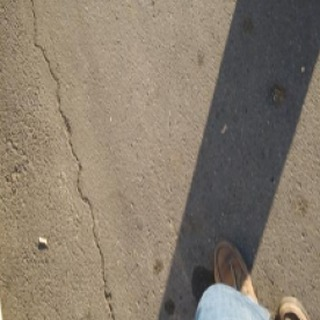
\includegraphics[width=\linewidth]{ombre_image.jpg}\par
        {\scriptsize Image}
      \end{minipage}\hfill
      \begin{minipage}[t]{0.48\linewidth}\centering
        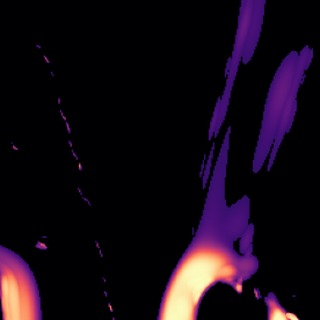
\includegraphics[width=\linewidth]{ombre_frangi.jpg}\par
        {\scriptsize Réponse Frangi}
      \end{minipage}\par\smallskip
      {\scriptsize Exemple de nos essais : l'ombre attire Frangi.}
    \end{column}
    \begin{column}{0.60\textwidth}
      \small\textbf{Faire prédire un poids par les caractéristiques SAM}\par\medskip
      \centering
      \resizebox{0.96\linewidth}{!}{% Proposition nouvelle : coefficient global appris, aucune mesure de performance.
\begin{tikzpicture}[every node/.style={font=\small,align=center},
  confidencebox/.style={draw=gris_fonce_inria,rounded corners=3pt,fill=gray!4,
    minimum height=.85cm,inner sep=5pt},
  flow/.style={-{Latex[length=2.4mm]},draw=gris_fonce_inria,line width=.9pt}]
  \node[confidencebox] (features) at (0,0) {Caractéristiques\\SAM : $\bar h(I)$};
  \node[confidencebox,draw=inria-rouge] (head) at (3.5,0) {Petite couche\\apprise};
  \node[confidencebox,draw=inria-rouge,fill=inria-rouge!5] (beta) at (6.65,0) {$\beta(I)$\\entre 0 et 1};
  \draw[flow] (features)--(head); \draw[flow] (head)--(beta);
\end{tikzpicture}
}
      \[\beta(I)=\mathrm{sigmoid}\!\left(w^\top\bar h(I)+b\right).\]
      {\scriptsize $\bar h(I)$ : moyenne des caractéristiques \textbf{avant} l'attention guidée.}
    \end{column}
  \end{columns}
  \vspace{0.16cm}
  \begin{center}
    \formulebox{\parbox{0.81\textwidth}{\centering\small
      $A_H(I)=\mathrm{softmax}\!\left(\text{scores visuels}+\beta(I)B_H(I)\right)$}}
  \end{center}
  \vspace{0.08cm}
  \small
  \begin{itemize}
    \setlength{\itemsep}{3pt}
    \item \textbf{Hypothèse :} moins de guidage quand Frangi gêne, notamment dans les ombres
      ou la granularité. Poids appris avec LoRA par la perte de segmentation.
    \item \textbf{Test :} sans biais / $\beta$ constant / $\beta(I)$.
      Comparer IoU, ruptures et faux raccords sur les mêmes images.
  \end{itemize}
  \vspace{0.06cm}
  {\footnotesize $B_H(I)$ dépend déjà de l'image ; on adapte ici \textbf{son poids}.
  Un poids global peut aussi réduire le guidage dans des zones utiles.}
\end{frame}

\end{document}
